\documentclass{article}
\usepackage{amsmath, amssymb, amsthm}
\usepackage{tikz}

\begin{document}

\title{Demostración de que ser Isomorfo es una Relación de Equivalencia}
\date{6 de septiembre de 2023}
\maketitle

Sea \( G \) una gráfica. Queremos demostrar que la relación "ser isomorfo" es una relación de equivalencia sobre gráficas. Recordemos que una relación de equivalencia debe cumplir con tres propiedades: reflexividad, simetría y transitividad.

\begin{enumerate}
    \item \textbf{Reflexividad:} Toda gráfica \( G \) es isomorfa a sí misma. 

    \textit{Demostración:}
    Supongamos que \( G \) es una gráfica con un conjunto de vértices \( V(G) \). Podemos definir un mapeo \( f: V(G) \to V(G) \) que es la función identidad, es decir, \( f(v) = v \) para todo \( v \) en \( V(G) \). Si \( u \) y \( v \) son vértices adyacentes en \( G \), entonces, bajo el mapeo \( f \), \( f(u) \) y \( f(v) \) también son adyacentes, ya que \( f \) es simplemente la función identidad. Por lo tanto, este mapeo preserva la estructura de la gráfica, lo que significa que \( G \) es isomorfa a sí misma.

    \begin{center}
    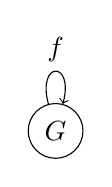
\begin{tikzpicture}
        \node[draw,circle] (A) at (0,0) {\( G \)};
        \draw[->,loop above] (A) to node[midway, above] {\( f \)} (A);
    \end{tikzpicture}
    \end{center}
    
    \item \textbf{Simetría:} Si una gráfica \( G \) es isomorfa a una gráfica \( H \), entonces \( H \) es isomorfa a \( G \).

    \textit{Demostración:}
    Supongamos que \( G \) y \( H \) son gráficas y que existe un isomorfismo \( f: V(G) \to V(H) \). Esto implica que \( f \) es una biyección que preserva la estructura de \( G \) en \( H \). Entonces, la función inversa \( f^{-1}: V(H) \to V(G) \) también será una biyección. Si dos vértices \( u \) y \( v \) en \( H \) son adyacentes, sus imágenes inversas bajo \( f^{-1} \) también serán adyacentes en \( G \), porque \( f \) es un isomorfismo. Por lo tanto, \( f^{-1} \) preserva la estructura de \( H \) en \( G \), y \( H \) es isomorfa a \( G \).

    \begin{center}
    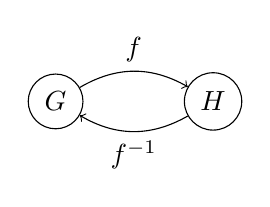
\begin{tikzpicture}
        \node[draw,circle] (A) at (0,0) {\( G \)};
        \node[draw,circle] (B) at (2,0) {\( H \)};
        \draw[->] (A) to[bend left] node[midway, above] {\( f \)} (B);
        \draw[->] (B) to[bend left] node[midway, below] {\( f^{-1} \)} (A);
    \end{tikzpicture}
    \end{center}

\item \textbf{Transitividad:} Si una gráfica \( G \) es isomorfa a una gráfica \( H \) y \( H \) es isomorfa a una gráfica \( I \), entonces \( G \) es isomorfa a \( I \).

    \textit{Demostración:}
    Supongamos que \( G, H, \) y \( I \) son gráficas, y existen isomorfismos \( f: V(G) \to V(H) \) y \( g: V(H) \to V(I) \). Queremos mostrar que existe un isomorfismo \( h: V(G) \to V(I) \). Definimos \( h = g \circ f \). Como \( f \) y \( g \) son biyecciones, su composición \( h \) también lo será. Si dos vértices \( u \) y \( v \) en \( G \) son adyacentes, entonces, bajo el mapeo \( f \), \( f(u) \) y \( f(v) \) serán adyacentes en \( H \). Dado que \( g \) es un isomorfismo, \( g(f(u)) \) y \( g(f(v)) \) serán adyacentes en \( I \). Por lo tanto, \( h \) preserva la estructura de \( G \) en \( I \), y \( G \) es isomorfa a \( I \).

    \begin{center}
    \begin{tikzpicture}
        \node[draw,circle] (A) at (0,0) {\( G \)};
        \node[draw,circle] (B) at (3,0) {\( H \)};
        \node[draw,circle] (C) at (6,0) {\( I \)};
        \draw[->] (A) to node[midway, above] {\( f \)} (B);
        \draw[->] (B) to node[midway, above] {\( g \)} (C);
        \draw[->, dashed] (A) to[bend south, distance=1cm] node[midway, below] {\( h \)} (C);
    \end{tikzpicture}
    \end{center}


\end{enumerate}

\end{document}
